\documentclass{article}\usepackage{float}\usepackage{listings} \usepackage{braket} \usepackage{amsmath,amssymb} \usepackage{geometry} \usepackage{graphicx} \usepackage{fancyvrb}\usepackage{braket} \usepackage{bm}\usepackage{hyperref} \usepackage{CJKutf8} \geometry{left=0.2cm,right=0.2cm,top=0.2cm,bottom=0.2cm} \renewcommand{\theequation}{\arabic{section}.\arabic{equation}} \renewcommand{\baselinestretch}{1.5}
\begin{document}
\begin{CJK}{UTF8}{gbsn}

  \section{深度学习与深层神经网路}
\label{sec:orgc7a7aa1}
\begin{enumerate}
\item 深度学习就是深层神经网络的代名词
\item 深度学习最重要的两个特性
\begin{itemize}
\item 多层
\item 非线性
\end{itemize}
\end{enumerate}

\subsection{线性模型的局限性}
\label{sec:org86497f4}

最早的神经网络采用线性模型

$$
  y=\sum_{i}w_ix_i+b
$$

$$
  a^{(1)}=xW^{(1)},y=a^{(1)}W^{(2)}
$$

$$
  y=(xW^{(1)})W^{(2)}\rightarrow y=x(W^{(1)}W^{(2)})=xW^{'}
$$

$$
  y=xW^{'}=\left[
\begin{array}{cc}
  x_1 & x_2 
\end{array}
\right]\left[
\begin{array}{c}
  W_1^{'} \\
  W_2^{'} 
\end{array}
\right]=\left[
\begin{array}{cc}
  W_{1}^{'}x_1 & W_2^{'} x_2
\end{array}
  \right]
$$

线性模型不能解决异或问题。

\begin{figure}[htbp]
  \centering
  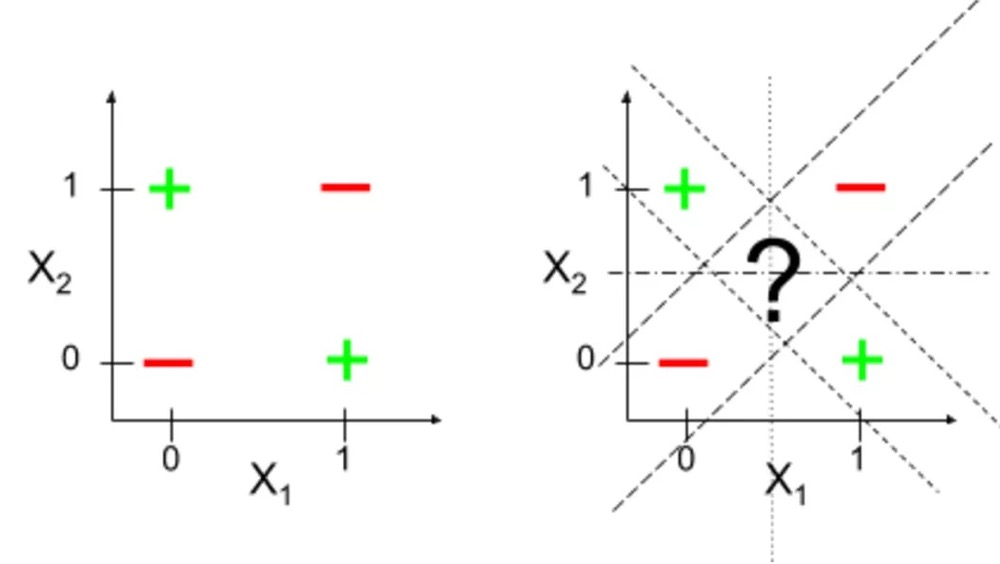
\includegraphics[width=0.6\linewidth]{xor.jpg}
\end{figure}	

\subsection{激活函数实现去线性化}
\label{sec:org420e81a}

如何做的?

\begin{figure}[H]
  \centering 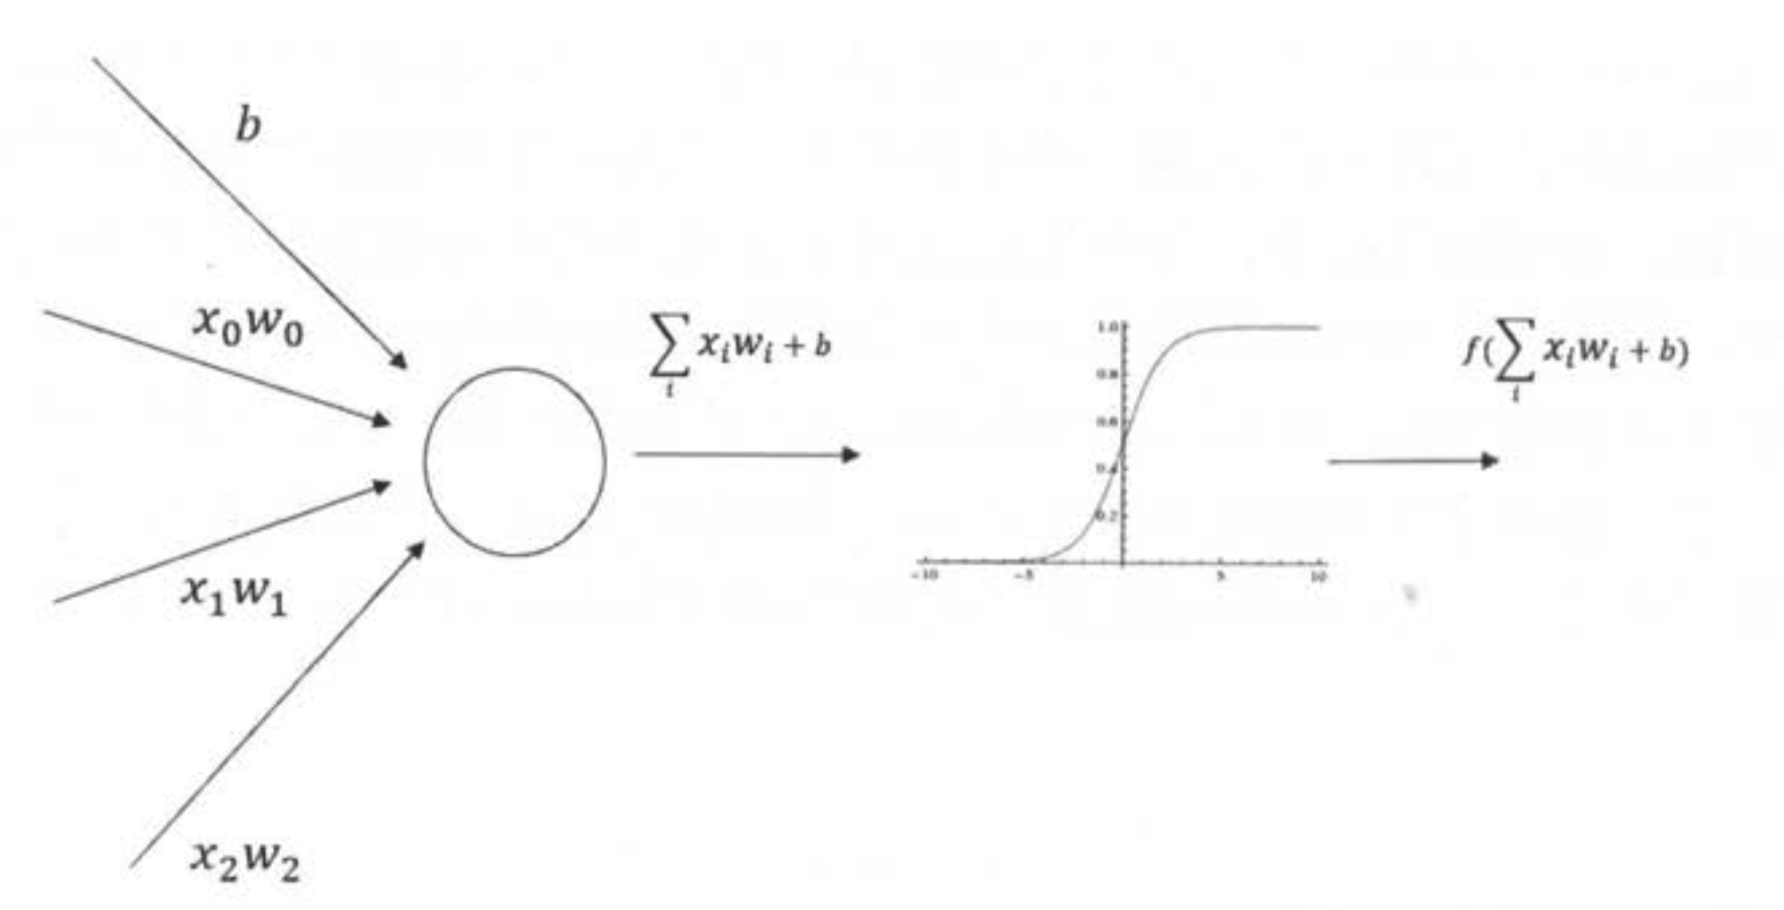
\includegraphics[width=0.6\linewidth]{nonlinear.png}
  \caption{加入非线性的激活函数图}
\end{figure}

\begin{displaymath}
  \begin{aligned} A_{1} &=\left[a_{11}, a_{12}, a_{13}\right]=f\left(x W^{(1)}+b\right)=f\left(\left[x_{1}, x_{2}\right]\left[\begin{array}{ccc}{W_{1,1}^{(1)}} & {W_{1,2}^{(1)}} & {W_{1,3}^{(1)}} \\ {W_{2,1}^{(1)}} & {W_{2,2}^{(1)}} & {W_{2,3}^{(1)}}\end{array}\right]+\left[\begin{array}{lll}{b_{1}} & {b_{2}} & {b_{3}}\end{array}\right]\right) \\ &=f\left(\left[W_{1,1}^{(1)} x_{1}+W_{2,1}^{(1)} x_{2}+b_{1}, W_{1,2}^{(1)} x_{1}+W_{2,2}^{(1)} x_{2}+b_{2}, W_{1,3}^{(1)} x_{1}+W_{2,3}^{(1)} x_{2}+b_{3}\right]\right) \\ &=\left[f\left(W_{1,1}^{(1)} x_{1}+W_{2,1}^{(1)} x_{2}+b_{1}\right), f\left(W_{1,2}^{(1)} x_{1}+W_{2,2}^{(1)} x_{2}+b_{2}\right), f\left(W_{1,3}^{(1)} x_{1}+W_{2,3}^{(1)} x_{2}+b_{3}\right)\right] \end{aligned}
\end{displaymath}

常用的激活函数

\begin{figure}[htbp]
  \centering 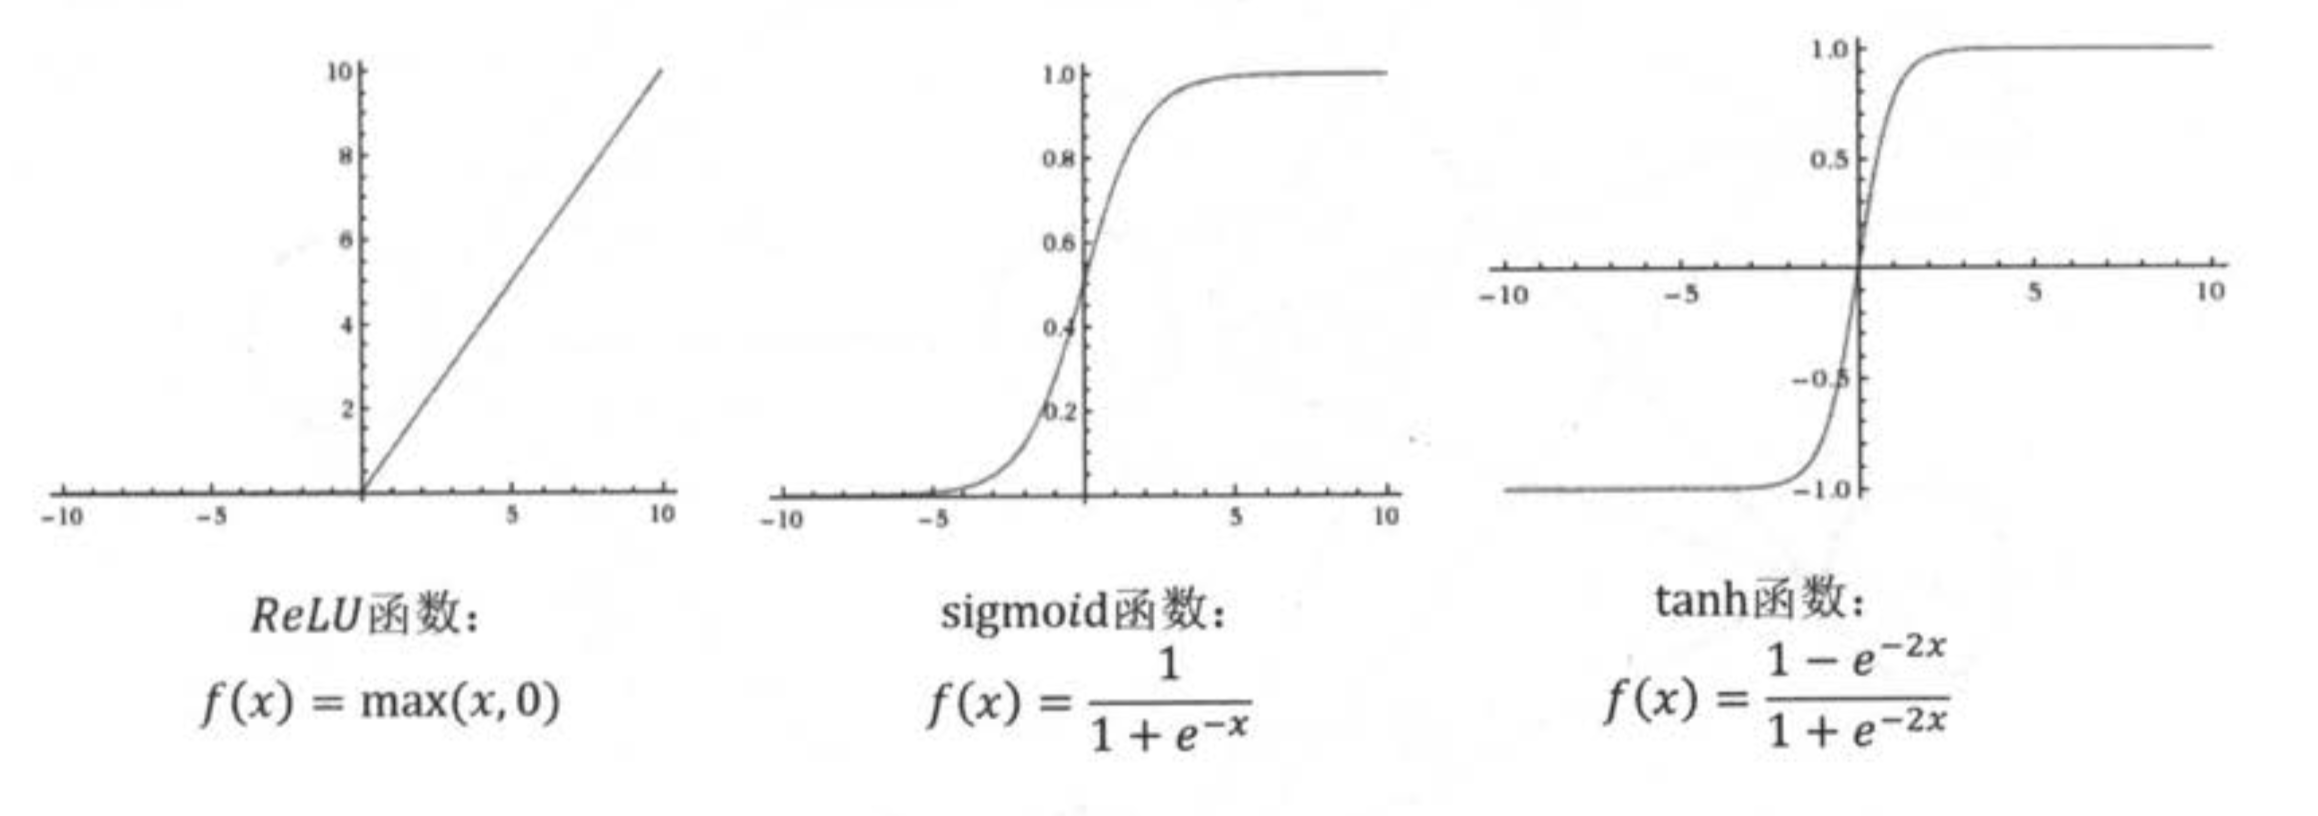
\includegraphics[width=0.8\linewidth]{act.png}
  \caption{常用的激活函数}
\end{figure}

\begin{lstlisting}[language=python]
  a = tf.nn.relu(tf.matmul(x,w1)+base1)
  b = tf.nn.relu(tf.matmul(a,w2)+base2)
\end{lstlisting}

\subsection{多层神经网络解决异或语言}
\label{sec:org32c6c09}

感知机理论上不可以的原因?(这个可以列一个专题来讲)FIXME 参考书籍《Perceptions:An Introtudction to Computational Geometry》 MIT Press,1969

\begin{figure}[H]
  \centering
  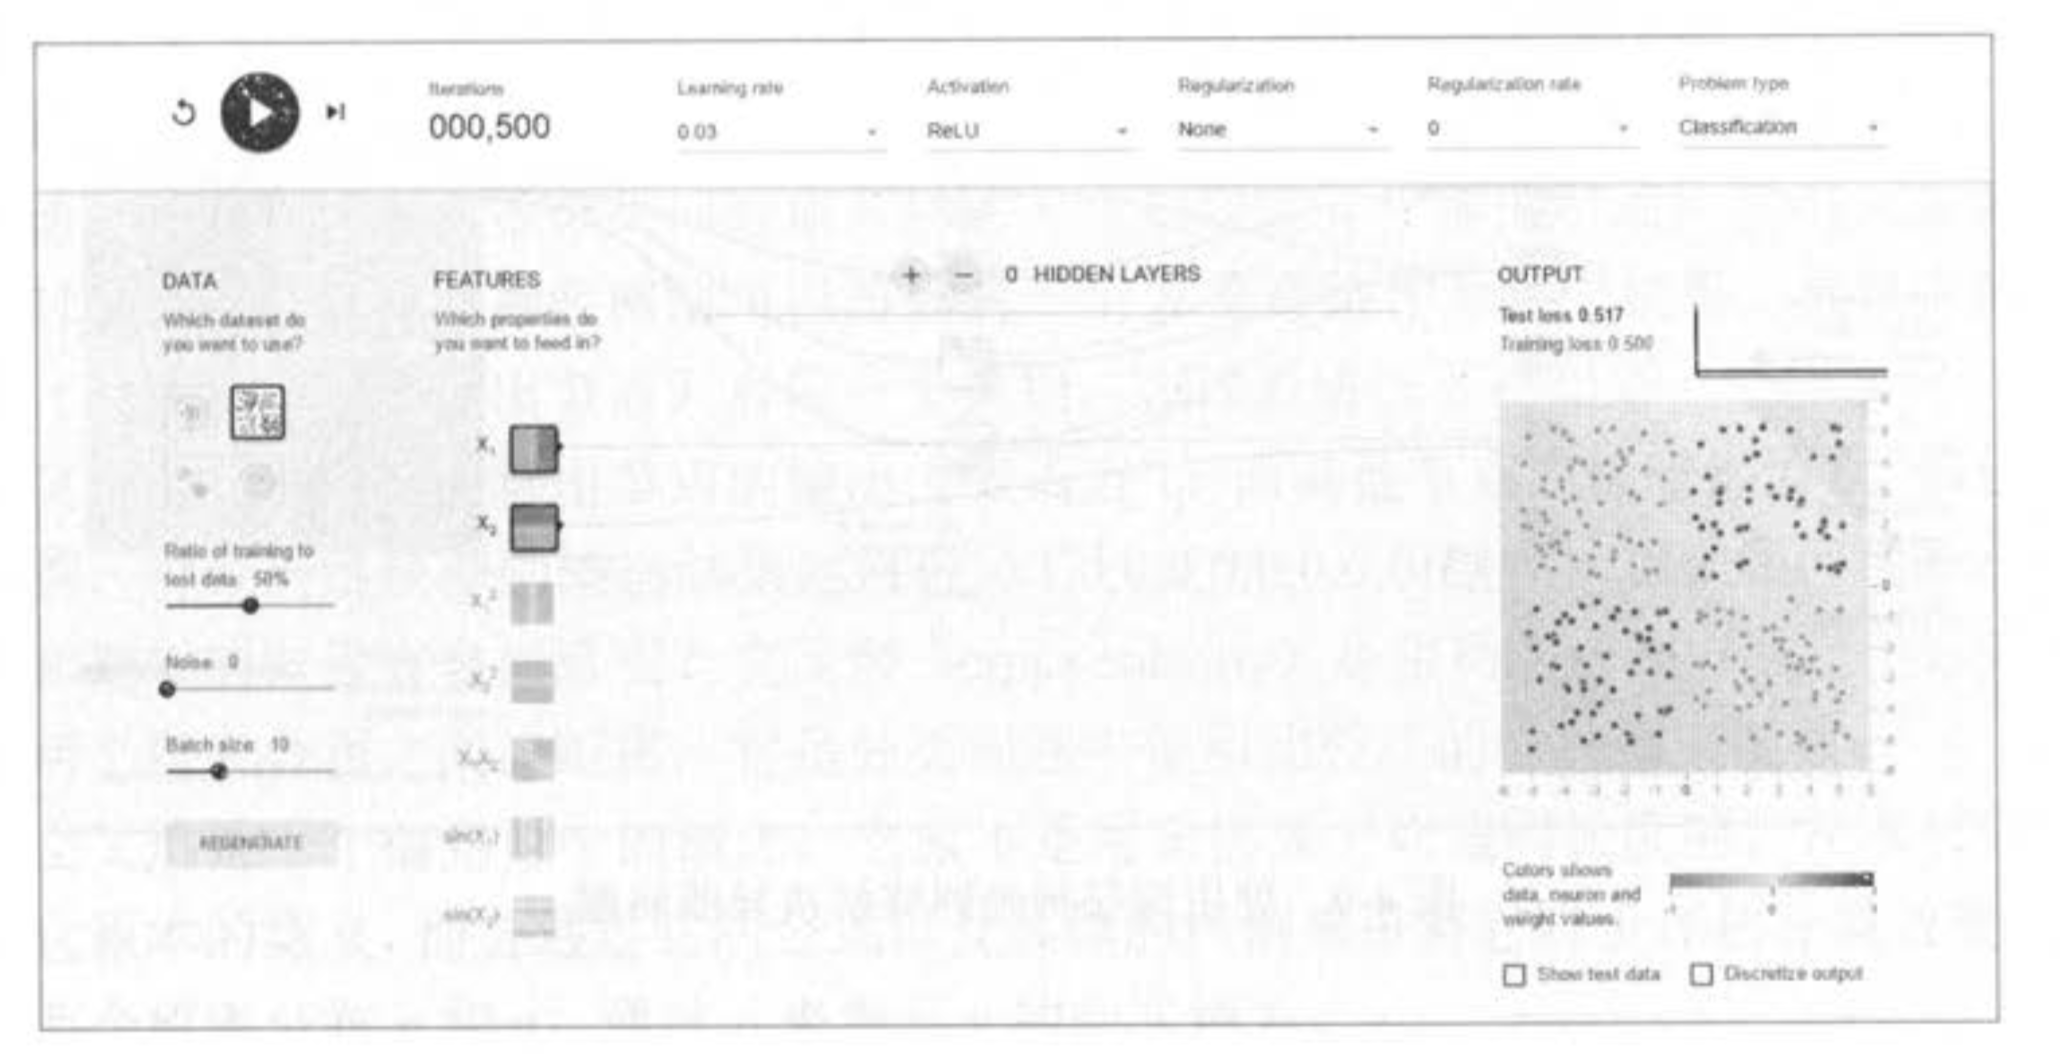
\includegraphics[width=0.8\linewidth]{perc.png}
  \caption{perception}
  \label{nosome}
\end{figure}

\begin{figure}[H]
  \centering
  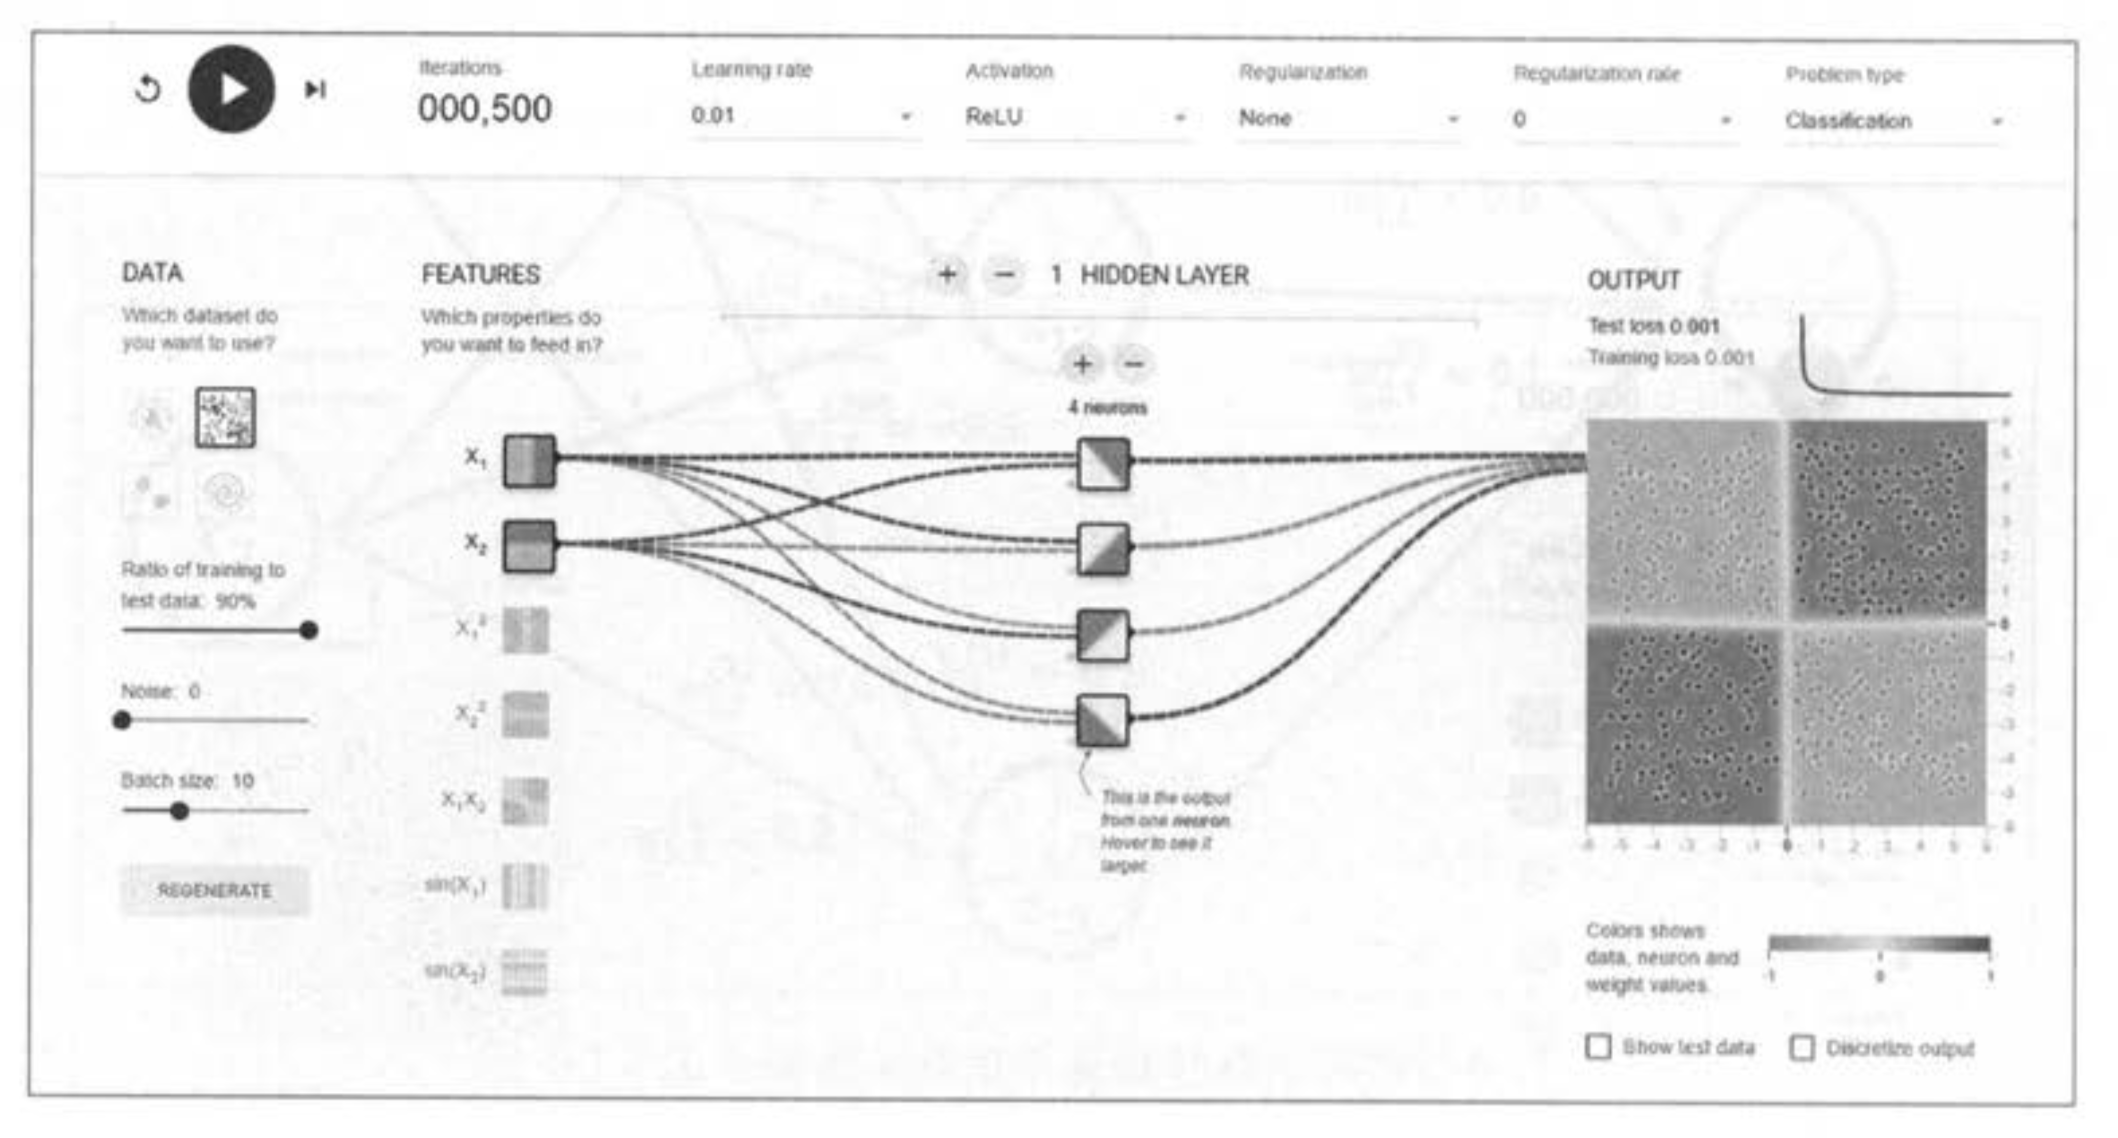
\includegraphics[width=0.9\linewidth]{deep.png}
  \caption{hidden layer for xor}
  \label{tdkks1}
\end{figure}

可以看到通过隐藏层,我们可以抽象出更为高维的信息。这些信息就可以用来分类数据。从而得到更好的分类结果。

\section{损失函数}
\label{sec:org8d79a79}

\subsection{经典损失函数}
\label{sec:org5239194}

神经网络如何输出多分类问题。比如3分类问题。苹果、香蕉、梨。

\begin{displaymath}
  \mbox{苹果}=\left(
    \begin{array}{c}
      1 \\
      0 \\
      0 
    \end{array}
  \right),\mbox{香蕉}=\left(
    \begin{array}{c}
      0 \\
      1 \\
      0 
    \end{array}
  \right),\mbox{梨}=\left(
    \begin{array}{c}
      0 \\
      0 \\
      1 
    \end{array}
  \right)
\end{displaymath}

如何比较输出值与预期值之间的差距? \textbf{交叉熵}。

交叉熵是用来衡量两个概率分布之间的距离的函数。它是分类问题中比较常见的损失函数。其定义为

\begin{displaymath}
  H(p,q)=-\sum_{x}p(x)log[q(x)]
\end{displaymath}

如何将神经网络的结果变成一个概率分布?使用softmax函数。

\begin{figure}[H]
  \centering
  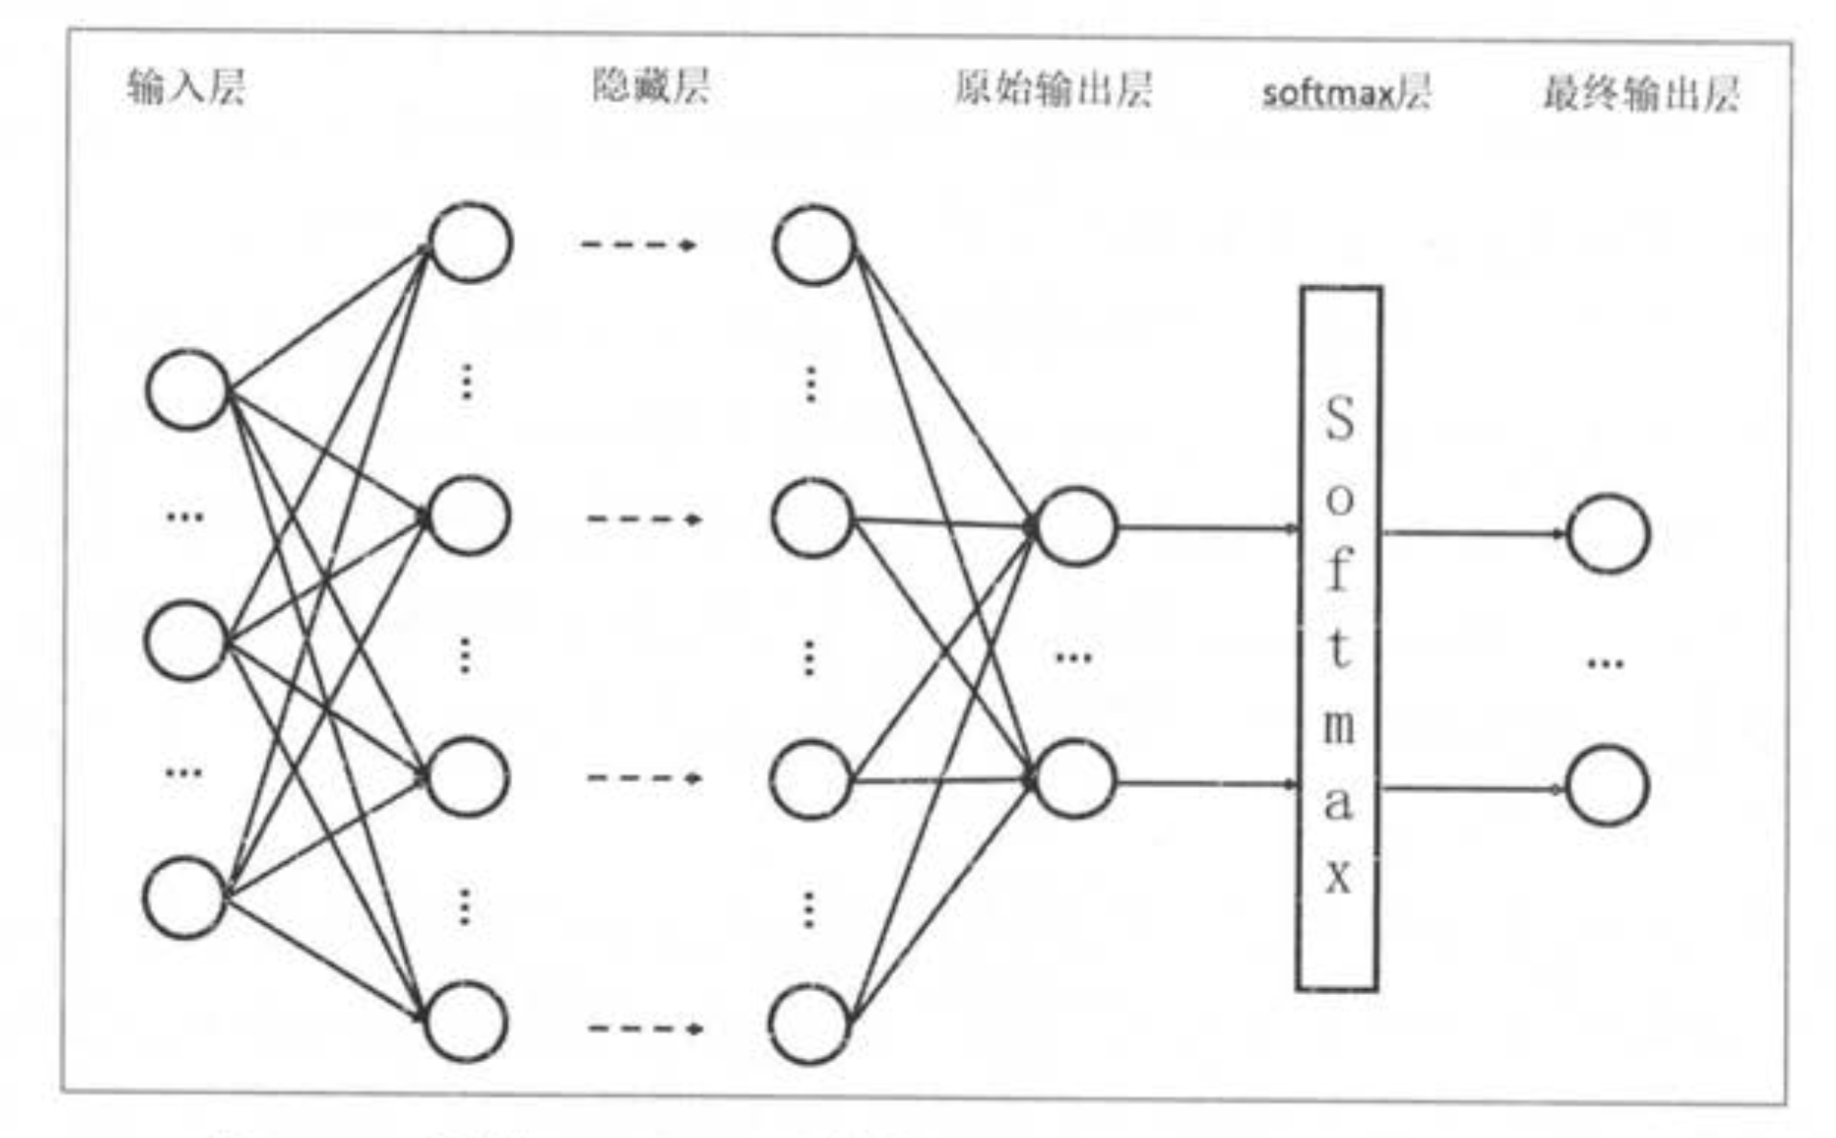
\includegraphics[width=0.6\linewidth]{softchange.png}
\end{figure}

加入神经网络的原始输出为$\{y_1,y_2,...,y_n\}$
\begin{displaymath}
  \operatorname{softmax}(y)_{i}=y_{i}^{\prime}=\frac{e^{y i}}{\sum_{j=1}^{n} e^{y j}}
\end{displaymath}

这个函数满足,概率分布的所有条件。这样就把神经网络的输出改成了一个概率分布。这样就可以计算交叉熵了。

但是需要注意的一点是交叉熵并不是对称的

\begin{displaymath}
  H(p,q)\neq H(q,p)
\end{displaymath}

比如我们可以这样来表述交叉熵$H(p,q)$,用q来刻画p的困哪程度。

\begin{lstlisting}[language=python]
  cross_entropy = -tf.reduce_mean(y_ * tf.log(tf.clip_by_value(y, le-10, 1.0)))
\end{lstlisting}

\begin{lstlisting}[language=python]
  v = tf.constant([[l.0, 2.0, 3.0], [4.0,5.0,6.0])) 
  print tf.clip_by_value(v, 2.5, 4.5).eval() 
  #Output[[2.5 2.5 3.][ 4. 4.5 4.5]]
\end{lstlisting}

\begin{lstlisting}[language=python]
  v = tf.constant([1.0, 2.0, 3.0]) 
  print tf.log(v) .eval( )
  #Output[ 0. 0.69314718 1.09861231]
\end{lstlisting}

\begin{lstlisting}[language=python]
  vl = tf.constant([[l.O, 2 .0], [3.0 , 4.0]]) 
  v2 = tf.constant([[5.0, 6.0], (7.0, 8.0]])
  print (vl *v2).eval()              #Output[[ 5. 12.] [ 21. 32.])
  print tf.matmul(vl , v2) .eval()   #Output[[ 19. 22.) [ 43. 50.)]
\end{lstlisting}

\begin{displaymath}
  \left(
    \begin{array}{cc}
      1 & 2 \\
      3 & 4 
    \end{array}
  \right)*\left(
    \begin{array}{cc}
      5 & 6 \\
      7 & 8 
    \end{array}
  \right)=\left(
    \begin{array}{cc}
      5 & 12 \\
      21 & 32 
    \end{array}
  \right)
\end{displaymath}



\subsection{自定义损失函数}
\label{sec:org2b3e954}

\section{神经网络优化算法}
\label{sec:org90a2418}
\section{神经网络进一步优化}
\label{sec:org5f20e0b}

\subsection{学习率的设置}
\label{sec:org11bb285}

\subsection{过拟合问题}
\label{sec:org9516d59}

\subsection{滑动平均模型}
\label{sec:org8864399}
  
  
\end{CJK}
\end{document}
